
\documentclass{scrartcl}
\usepackage[utf8]{inputenc}
\usepackage[T1]{fontenc}
\usepackage{verbatim}
\usepackage{enumitem}
\usepackage{graphicx}
\usepackage[ngerman]{babel}
\usepackage{hyperref}
\usepackage{xcolor}
\usepackage{pdfpages}
\setlength{\parindent}{0em} 
%TODO: maybe\setcounter{tocdepth}{4}
\setcounter{secnumdepth}{4}
\hypersetup{
    colorlinks,
    linkcolor={blue!65!black},
    citecolor={blue!50!black},
    urlcolor={blue!80!black}
}
\title{goApp Implementierung}
\author{Jörn Kussmaul, Katharina Riesterer, Julian Neubert,\\ Jonas Walter, Tobias Ohlsson, Eva-Maria Neumann}
\begin{document}
	\maketitle
	\newpage
	\tableofcontents
	\newpage

	\section{Einleitung}
	
	Der folgende Bericht beschreibt den Ablauf der Implementierungsphase der goApp, sowie Änderungen im Vergleich zum Pflichtenheft und dem Entwurf. Die im Entwurf festgelegten Klassen wurden zum Großteil so umgesetzt wie im Entwurfsdokument beschrieben, wobei einzelne Änderungen im nächsten Abschnitt beschrieben werden. Dabei ist Anzumerken, dass das Programmgerüst anhand der entworfenen UML-Diagramme erzeugt wurde. Die im Pflichtenheft festgelegten Kriterien wurden bis auf einige Wunschkriterien umgesetzt, worauf im Abschnitt "Kriterien" näher eingegangen wird.
	\newpage
	\section{Änderungen am Entwurf}
	Während der Implementierungsphase ergaben sich einige notwendige Änderungen gegenüber dem Entwurf. Diese sind im folgenden aufgeführt.
	
	\subsection{Server}
	\subsubsection{Servlet}
	\paragraph{GoServlet}
	Das GoServlet wird nicht mehr gebraucht und wird gelöscht. Die Funktionalität dieser Klasse wurde in das ParticipateServlet, bzw. EventServlet integriert.
	
	\paragraph{EventServlet}
	Die Methode getEvent wurde durch getParticipant ersetzt. Im momentanen Zustand braucht unsere App keine eigene Methode getEvents über die eventId, da die Events über die Gruppe gelesen werden. 
	Es fehlen nur die Informationen über die dazugehörigen Teilnehmer, weswegen dafür eine eigene Methode benötigt wird.
	
	\paragraph{GroupServlet}
	Aus getGroups wurde getMembers, da die Gruppe schon beim Erstellen auf den Client geholt wird und somit nur die Mitglieder der Gruppe gebraucht werden.
	
	\paragraph{LocationServlet}
	Die beiden Methoden setGPS, sowie setCluster werden zusammen über snycLocation aufgerufen. %TODO: warum 
	%TODO LocationServlet ruft immer beide Methoden auf (setGPS und getCluster)
	
	\paragraph{Participate Servlet}
	Die beiden Methoden accept und reject wurden durch die Methode setStatus ersetzt. Diese setzt den Status im Event-User Management, wodurch die Redundanz von zwei Methoden vermieden wird. Falls der Status Reject ist, wird der Teilnehmer gelöscht. 
		%Paticipate Servlet wird neu geschrieben
		%Paticipate: aus accept und reject wird setStatus
	
	\paragraph{UserServlet}
	Die Nutzer werden an den Client beim Einloggen bzw. Registrieren übermittelt und bis zum nächsten Einloggen gespeichert. Deswegen ist die Methode getUser überflüssig geworden.
	
	\paragraph{ServletUtils}
	Beim Implementieren der Servlets gibt es einige Schritte, die von jedem Servlet durchgeführt werden müssen. Dazu gehören zum Beispiel Methoden, um JSONObjekte aus der HTTP Anfrage auszulesen, oder das Verfassen der Antwort des Servers.
	Deswegen haben wir uns dazu entschieden eine statische Hilfsklasse zu nutzen, um diesen redundanten Code zu vermeiden. Außerdem definieren JSONObjekte eine wichtige Schnittstelle zum Client, da das Senden \& Empfangen von Informationen durch diese geregelt wird. In unserem Fall bleiben Änderungen der Schnittstelle somit lokal.
	
	\paragraph{JSONParameter}
	Wir brauchen viel mehr Parameter um die JSONObjekte zu erstellen, als in der Entwurfsphase angenommen. Außerdem gibt es ein weiteres Enum für die vom Client aufrufbaren Methoden, sowie eines für Fehlercodes. Die JSONParameter sind auf dem Client, sowie Server gleich. 
		
	\subsubsection{Algorithmus}	
	\paragraph{Clusteralgorithmus}
	Die Clusterfassade bietet nun neben der Methode getClusteredPoints auch die Methode getClusters und getCenter um direkt auf den Clusterer bzw. den Mittelpunktalgorithmus zugreifen zu können. Außerdem kann nun über den Konstruktor ein beliebiger Clusterer und Mittelpunktalgorithmus übergeben werden.
	
	\subsection{Model}
	\paragraph{User}
	Zusätzlich zu der id des Users in der Datenbank, die Google-Id als String.
	\paragraph{Group}
	Konstruktor hat nun zusätzlich den Gründer (User) als Parameter.
		\paragraph{Event}
	Konstruktor hat nun zusätzlich den Ort (Location), den Ersteller (User) und die Gruppe (Group) in welcher der Termin erstellt wird als Parameter.
	Die Zeit eines Events wird nicht als Time sondern als Timestamp gespeichert, dann ist das Datum mit dabei.

	\paragraph{Participant \& Status}
	Der Status in Participant ist zu einem Enum geworden.
	Der Status kann Invited, Participate, Started oder Rejected sein.	
	\subsection{Database Management}
	\paragraph{EventDeletionTimer}
	Läuft im Hintergrund und löscht Events nachdem deren Startzeitpunkt eine Stunde in der Vergangenheit liegt.
	\paragraph{LocationDeletionTimer}
	Läuft im Hintergrund und löscht veraltete Locations von Usern.
	\paragraph{GroupManagement}	
	Die Methoden getGroupsByMember,addMember und deleteMember wurden durch Methoden getGroups,add und delete in GroupUserManagement ersetzt.
	\paragraph{UserManagement}	
	Die Methode getUserByGoogleId kam hinzu um beim Starten der App den User der App zu laden.
	\paragraph{EventManagement}	
	\begin{itemize}
\item 	Die Methode updateStatus wurde durch die Methode updateStatus in EventUserManagement ersetzt.
\item 	Die Methoden getUserLocations und setClusterPoints wurden hinzugefügt um dem Algorithmuspaket den Zugriff auf die Daten zu erleichtern.
\item	Die Methode deleteOldEvents wurde hinzugefügt damit der EventDeletionTimer alte Events löschen kann.	
	\end{itemize}

	\paragraph{EventUserManagement}		
	
	\begin{itemize}
\item 		Die Methode getEventsByStatus wurde hinzugefügt damit die App die Events in getrennten Listen erhält.
\item Die Methoden getParticipant and getParticipants wurden hinzugefügt.
	\end{itemize}

		\paragraph{RequestManagement}		
	Die Methode getRequest wurde hinzugefügt. Diese gibt die Request aus der Datenbank mit der übergebenen userId und groupId zurück.

\subsection{Client}
	\subsubsection{View}
	Die GUI die der User zu Gesicht bekommt weist bis auf die Farbgebung kaum Unterschiede zum GUI Design aus der Entwurfsphase auf und an der Navigation zwischen den einzelnen Activities hat sich nichts geändert.
Im folgenden findet sich für jede Activity Änderungen welche Services von ihr gestartet werden können. 
	
	\paragraph{StartActivity}$~~$\\
	Zusätzliche Service Aufrufe:
	\begin{itemize}
	\item RequestService
	\end{itemize}
	Wegfallende Service Aufrufe:
	\begin{itemize}
	\item GroupService
	\end{itemize}

	\paragraph{GroupActivity}$~~$\\

	Zusätzliche Service Aufrufe:
	\begin{itemize}
	\item GroupService
	\end{itemize}
	Wegfallende Service Aufrufe:
	\begin{itemize}
	\item EventService
	\item GoService
	\end{itemize}

	\paragraph{EventActivity}$~~$\\

	Zusätzliche Service Aufrufe:
	\begin{itemize}
	\item EventService
	\end{itemize}
 

	\subsubsection{Controller}
	Im Entwurf haben wir unsere Services wie folgt beschrieben: 
\\
Sie alle erben von der Klasse IntentService, weshalb wir zusätzlich zum Konstruktor nur eine public Methode für jeden Service implementieren und zwar die Methode onHandleIntent(Intent intent). Weil diese Methode bei all unseren Services nur je nach Intent entscheidet, welche private Methode aufgerufen wird und das Ergebnis weiterleitet, haben wir uns dazu entschieden im folgenden nicht für jeden Service auf die besagte Methode einzugehen sondern jeweils die Methoden zu beschreiben welche durch onHandleIntent(Intent intent) aufgerufen werden, da dies unserer Meinung nach eine bessere Definition der Services Klassen liefert und damit für bessere Verständlichkeit sorgt.
\\
\\
Zwar existieren die Methoden die wir daraufhin beschrieben haben nach wie vor(bis auf Änderungen die ebenfalls in diesem Kapitel erläutert werden).
Allerdings sind die meisten der Methoden nicht mehr private sondern public. Bei den Services, wo dies der Fall ist werden besagte Methoden von den Activities direkt aufgerufen und erstellen den Intent, mit welchem erst im nächsten Schritt OnHandleIntent(Intent intent) des Services und damit ein neuer Thread gestartet wird. 
Die Funktionalität und der Rückgabewert der Services nach außen bleibt genau gleich, aber für die Activities ändert sich die Schnittstelle wie entsprechende Services aufgerufen werden.
So ist es jetzt schon bei Betrachtung des Codes einer Activity durch den expliziten Aufruf einer standardisierten Methode zum erstellen eines speziellen Intents klar, welche Daten der Client an dieser Stelle mit dem Server austauschen soll.    
\\
\\
Da die Servlets wie oben beschrieben verändert wurden mussten selbstverständlich auch die Services angepasst werden, da die Services des Clienten das Gegenstück zu den Servlets bilden wenn es um die Kommunikation zwischen Server und Clienten geht.
Da eine Veränderung des einen Teils zwangsläufig eine äquivalente Veränderung des Gegenstücks hervorruft wird hier nicht auf weitere Änderungen der Services eingegangen da diese aus Kapitel 2.1.1 hervorgehen.

\paragraph{UtilService} Die Klasse UtilService vereinigt Methoden die von verschiedene Services immer wieder aufgerufen werden müssen um JSON Parameter auszulesen. Um redundanten Code zu vermeiden haben wir deshalb auch auf dem Clienten diese statische Hilfsklasse eingeführt.  	

	\newpage
	\section{Kriterien}
	Im Pflichtenheft wurden Kriterien für unsere App definiert. Im folgenden unterteilen wir diese in erfüllt bzw. nicht erfüllt.

	
	\subsection{Erfüllte Kriterien}
		Alle Muss-Kriterien wurden erfüllt und außerdem noch einige von unseren Wunsch-Kriterien.
		
	\subsubsection{Kontoverwaltung}
	\begin{itemize}
		\item[FA10] Anmeldung eines Benutzers in der App über Google Services
		\item[FA20] Ersterfassung und Änderung des Benutzernamens
	\end{itemize}
	
	\subsubsection{Gruppenverwaltung}
	\begin{itemize}
		\item[FA30] Jeder Benutzer kann eine Gruppe erstellen
		\item[FA35] Ersterfassung und spätere Änderung des Gruppennamens durch den Gruppengründer
		\item[FA40] Gruppen können über den Gruppennamen gesucht werden
		\item[FA45] Benutzer können Beitrittsanfragen an eine Gruppe senden
		\item[FA50] Der Gruppengründer kann Beitrittsanfragen der Gruppe verwalten:
		\begin{itemize}
			\item Anfragen bestätigen, wodurch der Anfragende ein Mitglied der Gruppe wird und die Anfrage gelöscht wird
			\item Anfragen ablehnen, wodurch die Anfrage gelöscht wird
			\item Anfragen ignorieren, wodurch die Anfrage bestehen und sichtbar bleibt
		\end{itemize}
		\item[FA60] Der Gruppengründer kann Mitglieder aus der Gruppe entfernen
		\item[FA70] Die Gruppe kann durch den Gruppengründer gelöscht werden
		\item[FA80] Mitglieder der Gruppen, ausgenommen des Gruppengründers, können die Gruppe verlassen
		\item[FA90] Gruppenmitglieder können sich andere Gruppenmitglieder anzeigen lassen
	\end{itemize}
	
	\subsubsection{Terminverwaltung}
	\begin{itemize}
		\item[FA100] Jedes Mitglied einer Gruppe kann einen Termin erstellen
		\begin{itemize}
			\item Ersterfassung von Terminnamen, Terminzeit (in der Zukunft) und Terminort
			\item Visuelle Darstellung des gewählten Terminortes
		\end{itemize}
		\item[WFA105] Der Terminersteller kann den Terminnamen, Terminzeit und Terminort nachträglich ändern
		\item[FA110] Der Gruppenmittelpunkt wird anhand der Standorte aller Teilnehmer berechnet		
		\item[FA120] Jeder Termin wird jedem Gruppenmitglied angezeigt
		\item[FA130] Jedes Gruppenmitglied kann bei einem Termin zu- oder absagen
		
	\end{itemize}
	
	\subsubsection{Terminablauf}
	\begin{itemize}
		\item[FA140] Jeder Teilnehmer wird 30 Minuten vor Beginn des Termins benachrichtigt
		\item[WFA145] Teilnehmer werden auch bei geschlossener App benachrichtigt
		\item[FA150] Jeder Teilnehmer kann den Gruppenmittelpunkt ab 15 Minuten vor Beginn des Termins in einer Karte darstellen lassen
		\item[WFA155] Vom Gruppenmittelpunkt entfernte Teilgruppen  erhalten einen eigenen Standort 
	\item[WFA160] Teilnehmer können in der App anderen Teilnehmern mitteilen,
	\begin{itemize}
				\item dass sie bereits unterwegs sind
	\end{itemize}
		\item[FA170] Der Termin löscht sich nach der Dauer des Termins (standardmäßig 60 Minuten)
	\end{itemize}
		
		
	\subsubsection{Qualitative Anforderungen}
	Die Qualitativen Anforderungen beziehen sich auf unser Referenzgerät
	\glqq Samsung Galaxy S4\grqq  (GT-I9505) mit Android 5.0.1
	\begin{itemize}
		\item[QA10] Die App soll auf jede Anfrage in durchschnittlich unter 5 Sekunden reagieren
		\item[QA20] Die App fährt in durchschnittlich unter 10 Sekunden hoch
		%TODO: QA30 ??
		\item[QA30] Jede Funktion der App ist mit höchstens 5 Eingaben vom Startbildschirm der App zu erreichen
		\item[QA50] Unterstützt bis zu 50 Benutzer pro Gruppe
		\item[QA60] Jeder Benutzer kann in bis zu 20 Gruppen Mitglied sein
		\item[QA70] Der Server unterstützt das Anlegen von mindestens 30000 Benutzern
	\end{itemize}
	
	\newpage
	\subsection{Nicht erfüllte Kriterien}
	Wir haben es nicht geschafft alle Wunsch-Kriterien zu implementieren. Diese können allerdings in zukünftigen Updates der goApp noch erfüllt werden.
		\subsubsection{Kontoverwaltung}
		\begin{itemize}
			\item[WFA15] Der Benutzer kann zwischen Sprachen wählen
		\end{itemize}
		
		\subsubsection{Gruppenverwaltung}
		\begin{itemize}
			\item[WFA85] Der Gruppengründer kann seinen Status als Gruppengründer an ein Mitglied übergeben
			\item[WFA95] Gruppenmitglieder können die Teilnahmequoten anderer Gruppenmitglieder einsehen
		\end{itemize}

	\subsubsection{Terminverwaltung}
	\begin{itemize}
		\item[WFA105] Der Terminersteller kann den Termin löschen	
	\end{itemize}

	\subsubsection{Terminablauf}
	\begin{itemize}
	\item[WFA160] Teilnehmer können in der App anderen Teilnehmern mitteilen,
		\begin{itemize}
			\item dass sie zu spät kommen
			\item dass sie schon am Terminort angekommen sind
		\end{itemize}
			\item[WFA175] Die Dauer des Termins kann individuell festgelegt werden
	\end{itemize}	

	
	\newpage
	\section{Implementierungsplan}
	Während der Implementierungsphase haben sich einige Änderungen gegenüber unserem geplanten Verlauf ergeben.
	
	Unsere Woche Puffer am Ende haben wir durch eine Unterschätzung des Gesamtaufwandes doch gebraucht. Insbesondere die Arbeit auf dem Client wurde unterschätzt, da sich aufgrund der direkten Interaktion mit Benutzern viele Randfälle ergeben.
	
	Zusätzlich ergab sich eine große Änderung fast direkt zu Beginn, da wir gemerkt haben, da das HTTPConntectionPackage weniger Arbeit braucht als gedacht und wir somit die Aufgaben Database(Model) und Management ganz Jonas zugeordnet haben und Eva dafür an der Servlets gearbeitet hat. 
	
	\begin{figure}[h]
		\centering
		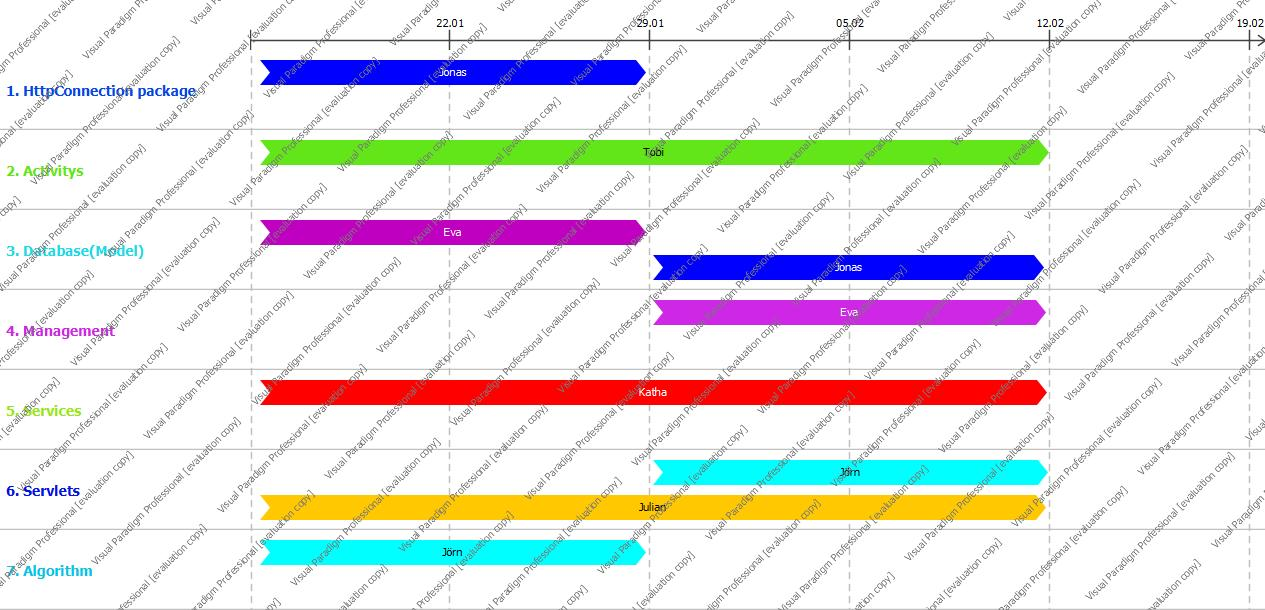
\includegraphics[width=0.8\textwidth]{ImplementationPlanDiagram.jpg}
		\caption{Das Implementierungsplandiagramm, vor der Implementierung.}
	\end{figure}

	\begin{figure}[h]
		\centering
		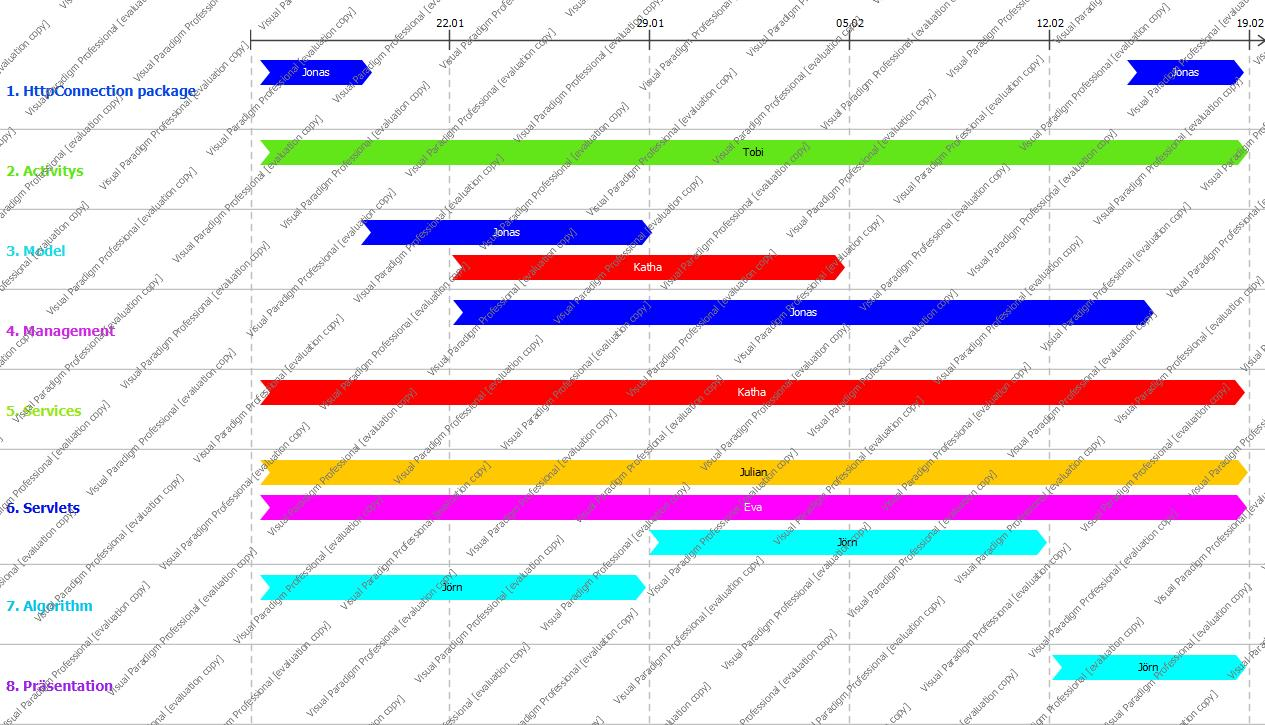
\includegraphics[width=0.8\textwidth]{ImplementationDiagram.jpg}
		\caption{Das Implementierungsdiagramm.}
	\end{figure}
	
	\newpage
	\section{Unit-Tests}
	Zum Testen unseres Codes haben wir Unit-Tests benutzt. In dieser Phase prüfen wir nur die Funktionalität. Weitere Tests zu Fehlerfällen folgen in der Testphase.
	\subsection{Server}
	\subsubsection{Datenbank}
	Um die Management Klassen, welche über Hibernate mit der Datenbank kommunizieren, zu testen haben wir auf dem PC eine MySQL-Datenbank erstellt. Jeder Testfall erstellt erst alle Daten, die er zum Testen benötigt, macht dann Datenbankabfragen und löscht die Daten wieder. Dadurch ist der Ausgangszustand für jeden Testfall immer klar definiert.
	\paragraph{DatabaseInitializer - DatabaseInitializerTest}	
	Testet ob das initialisieren der Datenbank klappt.
	\paragraph{EventDeletionTimer - EventDeletionTimerTest}	
	Die	EventDeletionTimerTest Klasse stellt sicher, dass das periodische löschen von veralteten Events funktioniert.
		\paragraph{LocationDeletionTimer - LocationDeletionTimerTest}	
	Die	LocationDeletionTimerTest Klasse stellt sicher, dass das periodische löschen von veralteten Locations funktioniert.
	\paragraph{EventManagement - EventManagementTest}	
	\subparagraph{public void testUpdate()}
	Der Test überprüft, dass die update Methode die Änderungen an einem Event in die Datenbank überträgt.	
	\subparagraph{public void testUpdateName()}
	Der Test überprüft, dass die updateName Methode nach der Änderung des Namens eines Events den neuen Namen in die Datenbank abspeichert.
	\subparagraph{public void testAdd()}
	Der Test stellt sicher, dass das hinzufügen eines Events funktioniert.
	\subparagraph{public void testDelete() }
	Der Test stellt sicher, dass das löschen eines Events funktioniert.
	\subparagraph{public void testGetCreator() }
	Der Test stellt sicher, dass beim Aufruf der getCreator Methode der richtige Ersteller zurück gegeben wird.
	\subparagraph{ public void testGetEvent() }
	Der Test stellt sicher, dass beim Aufruf von getEvent das richtige Event zurück gegeben wird.
	\subparagraph{public void testGetUserLocations() }
	Der Test stellt sicher, dass beim Aufruf der getGetUserLocations Methode alle Positionen der Eventteilnehmer zurück gegeben werden.
	\subparagraph{public void testSetClusterPoints()  }
	Der Test stellt sicher, dass beim Aufruf der setClusterPoints Methode die neuen Positionen korrekt in der Datenbank abgespeichert werden.
		
	\paragraph{EventUserManagement - EventUserManagementTest}
	\subparagraph{public void testAddUser()     }
		Der Test stellt sicher, dass das hinzufügen eines Users zu einem Event funktioniert.
	\subparagraph{    public void testUpdateStatus()  }
	Der Test überprüft, dass die update Methode die Änderungen in die Datenbank überträgt.	
	\subparagraph{ public void testGetParticipant()    }
		Der Test stellt sicher, dass beim Aufruf von getParticipant der richtige Participant zurück gegeben wird.
	\subparagraph{   public void testGetParticipants() }
		Der Test stellt sicher, dass beim Aufruf von getParticipants der richtigen Participants zurück gegeben werden.
	\subparagraph{    public void testDeleteParamsEventIdUserId()  }
	Der Test stellt sicher, dass das löschen eines Participants anhand der id des Users und des Events funktioniert.
	\subparagraph{   public void testDeleteParamsParticipantId()     }
	Der Test stellt sicher, dass das löschen eines Participants anhand der id des Participants funktioniert.
	\subparagraph{    public void testGetUsers()     }
	Der Test stellt sicher, dass beim Aufruf von getUsers die richtigen User zu einem Event zurück gegeben werden.
	\subparagraph{    public void testGetUserByStatus()     }
	Der Test stellt sicher, dass beim Aufruf von getUserByStatus alle User mit dem Status bei dem Event zurück gegeben werden.
	\subparagraph{    public void testGetEventsByStatus()     }
	Der Test stellt sicher, dass beim Aufruf von getEventsByStatus alle Events mit dem Status von einem User zurück gegeben werden.
	\subparagraph{    public void testGetEvents() }
	Der Test stellt sicher, dass beim Aufruf von getEvents die richtigen Events zu einem User zurück gegeben werden.

	\paragraph{GroupManagement - GroupManagementTest}
	    \subparagraph{ public void testAdd()  }
	Der Test stellt sicher, dass das hinzufügen einer Gruppe in der Datenbank funktioniert.
    \subparagraph{    public void testGetGroup()     }
	Der Test stellt sicher, dass beim Aufruf von getGroup die richtige Gruppe zurück gegeben wird.
    \subparagraph{public void testDelete()   }
	Der Test stellt sicher, dass das löschen einer Gruppe funktioniert.
    \subparagraph{    public void testGetEvents()   }
	Der Test stellt sicher, dass beim Aufruf von getEvents alle Events der Gruppe zurück gegeben werden.
    \subparagraph{    public void testUpdate()    }
   	Der Test überprüft, dass die update Methode die Änderungen in die Datenbank überträgt.	
    \subparagraph{    public void testGetGroupsByName()     }
	Der Test stellt sicher, dass die Methode getGroupsByName alle Gruppen aus der Datenbank deren Namen den übergebenen Namen enthält zurück gibt.
    \subparagraph{    public void testUpdateFounder()     }
   	Der Test überprüft, dass die updateFounder Methode den neuen Gründer in die Datenbank überträgt.	
    \subparagraph{    public void testUpdateName()     }
       	Der Test überprüft, dass die updateName Methode den neuen Namen in die Datenbank überträgt.	
       	
 	\paragraph{GroupUserManagement - GroupUserManagementTest}
	\subparagraph{    public void testAdd()     }
	Der Test stellt sicher, dass das hinzufügen eines Users zu einer Gruppe funktioniert.
    \subparagraph{    public void testDelete1()     }
	Der Test stellt sicher, dass man nicht den Gründer der Gruppe aus der Gruppe enfernen kann.
    \subparagraph{    public void testDelete2()     }
   	Der Test stellt sicher, dass das löschen eines Users aus einer Gruppe funktioniert.
    \subparagraph{    public void testGetGroups()     }
   	Der Test stellt sicher, dass die getGroups Methode alle Gruppen eines Users zurück gibt.
    \subparagraph{    public void testGetUsers()   }
   	Der Test stellt sicher, dass die getUsers Methode alle User einer Gruppe zurück gibt.
   	
 	\paragraph{RequestManagement - RequestManagementTest}
 	 \subparagraph{    public void testAdd()     }
	Der Test stellt sicher, dass das hinzufügen einer Request in der Datenbank funktioniert.
    \subparagraph{    public void testDeleteParamsRequestId()     }
	Der Test stellt sicher, dass das löschen einer Request anhand der und der Request funktioniert.
    \subparagraph{    public void testDeleteParamsGroupIdUserId()     }
    	Der Test stellt sicher, dass das löschen einer Request anhand der id des Users und der Gruppe funktioniert.
    \subparagraph{    public void testGetRequestByGroup()     }
   	Der Test stellt sicher, dass die getRequestByGroup Methode alle User, die eine Anfrage an die Gruppe gestellt haben, zurück gibt.
    \subparagraph{    public void testGetRequestByUser()    }
   	Der Test stellt sicher, dass die getRequestByUser Methode alle Gruppen, an die der User eine Anfrage gestellt hat, zurück gibt.
   	
	\paragraph{UserManagement - UserManagementTest}
    \subparagraph{    public void testAdd()   }
	Der Test stellt sicher, dass das hinzufügen eines Users in der Datenbank funktioniert.
    \subparagraph{    public void testDelete()   }
	Der Test stellt sicher, dass das löschen eines Users funktioniert.
    \subparagraph{    public void testGetUser()  }
   	Der Test stellt sicher, dass die getUser Methode den User mit der entsprechenden id zurück gibt.
    \subparagraph{ public void testGetUserByGoogleId()     }
   	Der Test stellt sicher, dass die getUser Methode den User mit der entsprechenden googleId zurück gibt.
    \subparagraph{    public void testUpdateLocation()     }
   	Der Test überprüft, dass die updateLocation Methode die neue Position in der Datenbank abspeichert.	
    \subparagraph{    public void testUpdate()     }
   	Der Test überprüft, dass die update Methode die Änderungen in die Datenbank überträgt.	
    \subparagraph{    public void testUpdateName()     }	
   	Der Test überprüft, dass die updateName Methode den neuen Namen in der Datenbank abspeichert.	
   	
   	
	\subsubsection{Algorithmus}
	Zum Einen wird hier überprüft ob der selbstgeschriebene Mittelpunktalgorithmus das korrekte Ergebnis ausgibt und auch Nullparameter richtig verarbeitet, zum Anderen wird die Klasse ClusterFacade durch Benutzung von Mockito auf die richtige Arbeitsweise überprüft, dabei wird die Richtigkeit der importierten Clusteralgorithmen vorausgesetzt. 
	\subsubsection{Servlet}
	Zum Testen der Servlets werden die jeweiligen Management Klassen der Datenbank, sowie HTTP requests gemockt.
	\paragraph{EventServlet}
	\subparagraph{public void testCreate()}
	Dieser Test prüft das erfolgreiche erstellen eines Events. 
	\subparagraph{public void testGetParticipates()}
	Dieser Test prüft das erfolgreiche Auslesen aller Teilnehmer der übergebenen Events.
	\subparagraph{public void testChange()}
	Dieser Test prüft das erfolgreiche Ändern des Namens des Events.
	\paragraph{GroupSearchServlet}
	\subparagraph{public void testMemberSearch()}
	Überprüft das erfolgreiche Einfordern einer Liste aller Gruppen, in denen ein gegebener Benutzer mitglied ist.
	\subparagraph{public void testNameSearch()}
	Überprüft das erfolgreiche Abrufen einer Liste aller Gruppen, in deren Name die gegebene Suchanfrage enthalten ist.
	\paragraph{LocationServlet}
	\subparagraph{public void testSyncPos()}
	Testet ob die gegebene Position des Benutzers in der Datenbank aktualisiert wird und der geclusterte Gruppenstandort des Events korrekt zurückgegeben wird.
	\paragraph{LoginServlet}
	Da jede der beiden Methoden auf den GoogleServer zum Verifizieren des GoogleTokens zugreift und man dies nicht testen kann, wird dieses Servlet erst manuell über den Client mit einem echten GoogleAccount getestet. Dort funktioniert das Registrieren, sowie auch Anmelden.
	\paragraph{ParticipateServlet}
	\subparagraph{public void testSetStatus()}
	Testet das korrekte setzen des Status' auf "teilnehmen".
	\paragraph{GroupServlet}
	\subparagraph{public void testGroupCreating()}
	In diesem Test wird eine Gruppe erstellt.
	\subparagraph{public void testGroupDeleting()}
	Dieser Test versucht eine Gruppe zu entfernen.
	\subparagraph{public void testNameChanges()}
	Hier wird eine Anfrage vom Client zum Ändern des Namens einer Gruppe simuliert.
	\subparagraph{public void testMemberKicking()}
	Es wird das Entfernen von Mitgliedern aus einer Gruppe getestet.
	\subparagraph{public void testEventRequesting()}
	Diese Methode testet das Abfragen aller zu einer Gruppe und einem Benutzer zugehörigen Events. Hierbei werden die Events, die bereits vom Nutzer bestätigt wurden separat von denen, auf die der Nutzer noch antworten muss, zurückgegeben.
	\subparagraph{public void testMemberRequesting()}
	Es wird das Abrufen einer Liste mit allen Mitgliedern einer Gruppe getestet.
	\subparagraph{public void testFounderChanging()}
	In diesem Test wird der founder einer Gruppe aktualisert.
	\paragraph{RequestSearchServlet}
	\subparagraph{public void testGetRequestsByGroup()}
	Dieser Tests prüft das erfolgreiche holen aller Gruppen, zu dem von einem gegeben User, eine Anfrage existiert.
	\subparagraph{public void testGetRequestsByUser()}
	Dieser Tests prüft das erfolgreiche holen aller Nutzer, zu dem von einem gegeben Gruppe, eine Anfrage existiert.
	\paragraph{RequestServlet}
	\subparagraph{public void testCreate()}
	Dieser Test prüft das erfolgreiche Anlegen eines neuen Requests.
	\subparagraph{public void testAccept()}
	Dieser Test prüft das erfolgreiche Akzeptieren eines Requests.
	\subparagraph{public void testReject()}
	Dieser Test prüft das erfolgreiche Ablehnen eines Requests.
	\paragraph{ServletUtils}
	In den ServletUtils werden die 3 Methoden testIsUserAlreadyRegistrated(), testGetGoogleIdByToken() und testGetGoogleNameByToken() nicht getestet, da diese auf GoogleServer zugreifen und ein gültiges GoogleToken benötigen.
	\subparagraph{public void testCreateJSONParticipate()}
	Dieser Test prüft das erfolgreiche Erstellen eines JSONObjektes aus einem Participate Objekt.
	\subparagraph{public void testCreateJSONListPart()}
	Dieser Test prüft das erfolgreiche Erstellen eines JSONObjektes
	\subparagraph{public void testCreateJSONEventID()}
	Dieser Test prüft das erfolgreiche Erstellen eines JSONObjektes mit nur der EventID aus einem Event Objekt.
	\subparagraph{public void testCreateJSONEvent()}
	Dieser Test prüft das erfolgreiche Erstellen eines JSONObjektes aus einem Event Objekt.
	\subparagraph{public void testCreateJSONLocation()}
	Dieser Test prüft das erfolgreiche Erstellen eines JSONObjektes aus einem Location Objekt.
	\subparagraph{public void testCreateJSONGroup()}
	Dieser Test prüft das erfolgreiche Erstellen eines JSONObjektes aus einem Group Objekt.	
	\subparagraph{public void testCreateJSONUser()}
	Dieser Test prüft das erfolgreiche Erstellen eines JSONObjektes aus einem User Objekt.	
	\subparagraph{public void testCreateJSONListEvent()}
	Dieser Test prüft das erfolgreiche Erstellen eines JSONObjektes aus einem User Objekt.
	\subparagraph{public void testCreateJSONDoubleListEvent()}
	Dieser Test prüft das erfolgreiche Erstellen eines JSONObjektes aus 2 Listen mit Event Objekten
	\subparagraph{public void testCreateJSONListUsr()}
	Dieser Test prüft das erfolgreiche Erstellen eines JSONObjektes aus einer Liste von User Objekten.
	\subparagraph{public void testCreateJSONListGrp()}
	Dieser Test prüft das erfolgreiche Erstellen eines JSONObjektes aus einer Liste von Group Objekten.
	\subparagraph{public void testCreateJSONGroupID()}
	Dieser Test prüft das erfolgreiche Erstellen eines JSONObjektes mit nur der GroupID aus einem Group Objekt.	
	\subparagraph{public void testCreateJSONListLoc()}
	Dieser Test prüft das erfolgreiche Erstellen eines JSONObjektes aus einer Liste von Location Objekten.
	\subparagraph{public void testCreateJSONError() }
	Dieser Test prüft das erfolgreiche Erstellen eines JSONObjektes aus einem ErrorCodes Objekt.

	\paragraph{UserServlet}	
	\subparagraph{public void testChangeName()}
	Dieser Test überprüft das erfolgreiche Ändern des Namens des Nutzers.
	
	\subsection{Client}
	\subsubsection{HTTPConnection}
	\subparagraph{public void testSendGetRequest()}	
	Der Test überprüft, dass die get-Anfragen an den Server funktionieren.
	\subparagraph{public void testSendPostRequest()}
	Der Test überprüft, dass die post-Anfragen an den Server funktionieren.
	\subparagraph{public void testConnectionFailed()}
	Der Test überprüft, dass wenn ein Service nicht erreichbar ist ConnectionFailed zurück gegeben wird.
	\subsubsection{View}
	Für die View haben wir keine Testfälle implementiert da diese sich besser "von Hand" testen lässt. Durch einfaches benutzen der goApp können wir überprüfen, dass die View sich so verhält wie wir als Implementierer es erwarten.
Auch in der nächsten Phase werden wir die View nicht mit klassischen Unit-Tests abdecken, sondern durch Monkey-Tests die Robustheit unserer Applikation bei Eingaben jeglicher Art sicherstellen.
Ebenfalls wird die goApp an die ersten User verteilt um uns Feedback über die hoffentlich intuitive Bedienbarkeit der GUI einzuholen.

	\subsubsection{Controller}
	Es ist nicht möglich Intent Services mit Unit-Tests zu testen.  Da unser Controller wie im Entwurf beschrieben nur Intent Services implementiert existieren hier also keine Unit-Tests.
Allerdings ist der Großteil der Logik in die Klasse UtilService ausgelagert. 

	\paragraph{UtilService}
	\subparagraph{public void getGroups()}
	Dieser Test überprüft das erfolgreiche erstellen eines Group Arrays aus einem JSON Objekt.
	\subparagraph{public void getUsers()}
	Dieser Test überprüft das erfolgreiche erstellen eines User Arrays aus einem JSON Objekt.
	\subparagraph{public void getParticipants()}
	Dieser Test überprüft das erfolgreiche erstellen eines User Arrays, aus einem JSON Objekt wobei hier jeder User einen Status hat.
	\subparagraph{public void getLocations()}
	Dieser Test überprüft das erfolgreiche erstellen eines Location Arrays aus einem JSON Objekt.
	\subparagraph{public void isErrorTrue()}
	Dieser Test überprüft das erkennen von Fehlern.
	\subparagraph{public void isErrorFalse()}
	Dieser Test überprüft das erkennen einer Fehlerfreien Kommunikation mit dem Server. 
	\subparagraph{public void getError()}
	Dieser Test überprüft ob ein Error Code als der richtige erkannt wird.
	\subparagraph{public void getEvents()}
	Dieser Test überprüft das erfolgreiche erstellen eines Event Arrays aus einem JSON Objekt.
	
\end{document}
